\section{performance evaluation}
\label{sec:performance evaluation}
In this section, we first present the simulation results of applying our algorithm to find the SRLG disjoint paths, then the results on finding the SRNG disjoint paths. As we could not find any topology trace data that contain SRLG (or SRNG), we generate a synthesized data  set by injecting SRLGs (or SRNGs) into a Huawei topology trace. The topology trace has $\TopoNum$ different topologies with various number of nodes, links, link weights (\rev{representing the link delay} or other parameter). The source codes of our algorithms and the synthesized topology trace sets can be downloaded from the github website \cite{code}.
\note{Does Huawei allow to publish their data?}

\subsection{Simulation of finding the SRLG disjoint paths}
\subsubsection{Simulation setup}
\label{subsub:Simulation setup}
 Two kinds of SRLG are generated in our simulation, the star-style and the non-star-style. In Optical Networks, SRLG is star-style, while in other networks such as an overlay network, SRLG can be non-star-style. Each SRLG group is generated by randomly selecting 2-5 links. Table \ref{tab:AllSample} shows the basic network setting (number of nodes, links) in these $\TopoNum$ topologies. Based on the topology trace, we randomly generate SRLG groups, with the number of SRLG graphs injected and the SRLG edge ratio (defined as $\frac{{No.SRLG \  {\rm{ }}edges}}{{Total \  {\rm{ }}No.edges}}$) shown on the 3rd and 4th rows of the table.



%The github website \cite{code} support complete experimental code and experimental topology data.}


%We use the topology without \revtao{SRLG's information} trace published by Huawei to evaluate the performance of our proposed scheme (named by \CI). As introduced in related work, unavoidable traps are caused by the topology constraints. The topology trace provided by Huawei does not have unavoidable traps. That is, although a BP path may not be able to be found for an AP path, \revtao{there must exist two edge-disjoint paths in the network between the source node to the destination node}. As the topology trace has $\TopoNum$ different topologies with various number of nodes, links, link weights\revtao{(represent link's delay or other parameter), we generate a simple sample topology as shown in Fig.\ref{fig:CompositeGraph}(c) which include SRLG's information and all algorithm process this small-scale sample topology then happen trap problem , with that we random generate SRLG groups in huawei's topology, these SRLG groups is 2\%-5\% of edge number, we assemble the small-scale topology with huawei's topology and generate experimental processing topology's data finally}, we compare our algorithm with other peer algorithms using each topology. Table \ref{tab:AllSample} shows the basic network setting in these $\TopoNum$ topologies. After normalizing the result in each topology, we take the average of the normalized results as the final simulation result \revtao{according to min-max normalization \cite{han2011data}. In Fig.\ref{fig:normalization hop},\ref{fig:normalization runtime} we set every algorithm's weight or hop path of AP, BP and AP+BP as a group data to be normalized, and average every algorithm's weight or hop path of AP, BP and AP+BP of the $\TopoNum$ normalized data. In Fig.\ref{fig:normalization runtime} we set every core's situation's runtime of four alogrihtm as a group to be normalized, and the like in Fig.\ref{fig:Speedup},\ref{fig:Efficiency},\ref{fig:Multiple}, and average runtime or other measure parameter of the $\TopoNum$ normalized data.. The github website \cite{code} support complete experimental code and experimental topology data. In most sample, KSP algorithm can not get any solution. And ILP and IQCP may not calculate the solution in constraints of Integer Programming in some special samples}.



\begin{table*}[tp]
\caption{$\TopoNum$ different topologies.}
  \centering
\footnotesize{  \begin{tabular}{*{18}{c}}
\toprule
Topology & 1 & 2 & 3 & 4 & 5 & 6& 7   \\
\midrule
Node    &     527&      521    &      521     &    2023             &     451     &     521     &     449       \\
Edge   &    4158 &  4052     &    4152      &   4142          &       2780   &      4052   &      2778    \\
%Graph density  & 1.5\% &    1.49\% &   1.52\%  &  0.1\%  &   0.10\% &   1.41\%  &  1.5\% &   1.38\%   \\
No.SRLG & 132 &  86   &  89  &  207        & 210  &  128  &   88    \\
SRLG edge ratio & 9.66\% & 6.16\% &   6.18\% &   14.94\%    &   22.55\%  &  9.65\% &   9.53\%     \\
\bottomrule
\end{tabular}
}

\label{tab:AllSample}
\end{table*}
For performance comparisons, besides our scheme (named by \CI), we also implemented other four SRLG-disjoint routing algorithms as follows:


\begin{enumerate}
  \item ILP: The work in \cite{hu2003diverse}  aims to find SRLG-disjoint paths through an ILP formulation such that the total weight of the two paths is minimized. We are not aware that other studies look for the Min-Min SRLG-disjoint paths through ILP formulation. Therefore, following \cite{hu2003diverse}, we formulate  our Min-Min SRLG-disjoint routing problem by changing the objective function.
  \item IQCP: As any $0-1$ integer linear program where all variables are either 0 or 1,  ILP can be formulated as a quadratically constrained program. Different from ILP, we also model Min-Min SRLG-disjoint routing problem through the Integer Quadratic Constraints Program (IQCP) \cite{hu2003diverse}.
  \item KSP \cite{eppstein1998finding}: It finds the first $K$ shortest paths between the source and the destination as candidate APs, and then tests them one by one in the increasing order of their costs to see if it has a corresponding (SRLG-disjoint) BP, until such a BP is found.
  \item CoSE \cite{rostami2007cose}: When an AP encounters a trap problem, CoSE tries a simple and exhaustive search to find a SRLG set that no AP going through the SRLG set can find the SRLG-disjoint BP path. Based on the SRLG set, it partitions the original problem  and designs an algorithm to search for the SRLG disjoint path pair.
\end{enumerate}
%\rev{As constraints of ILP equation for keeping linear calculation is $\sum\limits_{1\leq i \leq \chi} |\mathbb{R}_{r_i}|^2$ more than that of IQCP, ILP can be formulated as a quadratically constrained program so that reduce the quantity of constraints. As ILP}, we also model Min-Min SRLG-disjoint routing problem through the Integer Quadratic Constraints Program (IQCP) \rev{based on} \cite{hu2003diverse}.
The first two (ILP and IQCP) are based on integer program models. In our implementation, the tool GUROBI 7.0 \cite{optimization2012gurobi} is employed to resolve these two integer program problems.  Six performance metrics are applied to evaluate the performance of different SRLG-disjoint routing algorithms:

\textbf{Path weight}: is the sum of the link weight in the path.

\textbf{Path hop}: the number of hops in the path.

\textbf{Runtime}: the average number of \revtao{normalized milliseconds} taken for SRLG-disjoint path finding.

\textbf{Algorithm speedup}: Given the computation time under two different  algorithms ($alg_1$ and $alg_2$), denoted as $T_1$ and $T_2$, the algorithm speedup in the computation time of the $alg_2$ with respect to the $alg_1$: ${S_{1 - 2}} = T_1/T_2$.

\textbf{Core speedup}: The core speedup \cite{grama2003introduction} of a parallel program is typically defined as $S_P=\frac{T_1}{T_p}$,
where $p$ is the number of processor cores and $T_1$ and $T_p$ denote the running time on 1 core and $p$ cores, respectively.

\textbf{Efficiency}: is defined \cite{grama2003introduction} as $E_p=\frac{S_p}{p}=\frac{T_1}{pT_p}$,it is typically reported as a percentage in the range (0, 1].

All simulations are run on a linux server, which is equipped with Intel(R) Xeon(R) CPU E5-2620 0 \@ 2.00GHz (24 Cores) and 32.00GB RAM. To measure the computation time, we insert a timer to all the implemented algorithms.

All algorithms are implemented using 7 topologies. For the reason of space saving, we take the average results of different topologies as the final results. Specially, as different topologies may result in different performance value ranges, for each topology, we normalize the performance value of Weight, Hop and Runtime under different algorithms according to min-max normalization \cite{tax2000feature}. We take the average of the normalized results as the final simulation results. For other performance \rev{metrics} (algorithm speedup, core speedup, and efficiency), according to \rev{their definitions}, we use the normalized Runtime \rev{values to derive their values. }
\subsubsection{Simulation result}
\label{subsubsec:Simulation result}
Among \del{the} five SRLG disjoint routing algorithms, only CoSE and our SCLS are parallel algorithms. Although ILP, IQCP and KSP are not parallel algorithms, we still implement them as we want to present the speed gain obtained by our design.
From the analysis in Section \ref{subsec:Complexity analysis}, under KSP, the computation complexity to find the first $K$ shortest paths is $K\times ((|\mathbb{E}|+|\mathbb{V}|)\times log(|\mathbb{V}|))$ , which would be large with the worst $K=2^{|\mathbb{E}|}$.
% where $K$ is the number of first  shortest paths that should be tested before finding the SRLG disjoint BP.}
 Consistent with the analysis, when we run KSP using the $\TopoNum$ topologies, no simulation results can be returned within 1 hour, while others can return results within 11 seconds. Long computation time makes KSP difficult to use in practice. Therefore, we do not provide the simulation results under KSP.

\begin{itemize}
  \item Path Weight
\end{itemize}

Fig.\ref{fig:normalization weitgh sum} shows the weight of AP, BP, and the sum of both AP and BP. Obviously, all implemented algorithms \CI, CoSE, ILP and IQCP achieve the same AP weight, but different BP weights thus different sum weights of AP and BP. As all the algorithms solve the same Min-Min SRLG-disjoint routing program, although they find different SRLG-disjoint path pairs, they can all achieve the goal of finding the  AP with the same least weight.
As \CI, CoSE find the  BP based on a shortest path algorithm (such as Dijkstra), they also find the BP path with the same weight. However, the two ILP-based algorithms, ILP and IQCP, focus on minimizing the weight of AP but find any BP that is SRLG-disjoint with AP, the BP paths searched by these two algorithms are different.



\begin{figure*}[tp]
\centering
\subfigure[Path weight]{
\label{fig:normalization weitgh sum}
\includegraphics[width=0.22\textwidth]{franz/weight}}
\subfigure[Path hop]{
\label{fig:normalization hop}
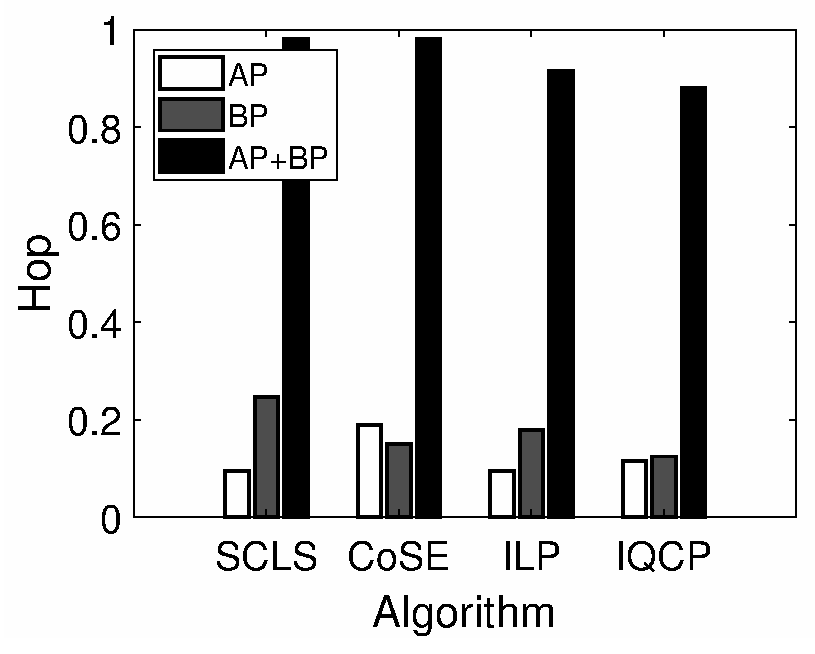
\includegraphics[width=0.22\textwidth]{franz/hop}}
\subfigure[Runtime]{
\label{fig:normalization runtime}
\includegraphics[width=0.22\textwidth]{franz/runtime}}
\subfigure[Runtime without CoSE]{
\label{fig:Runtime_noKSP_noCOSE}
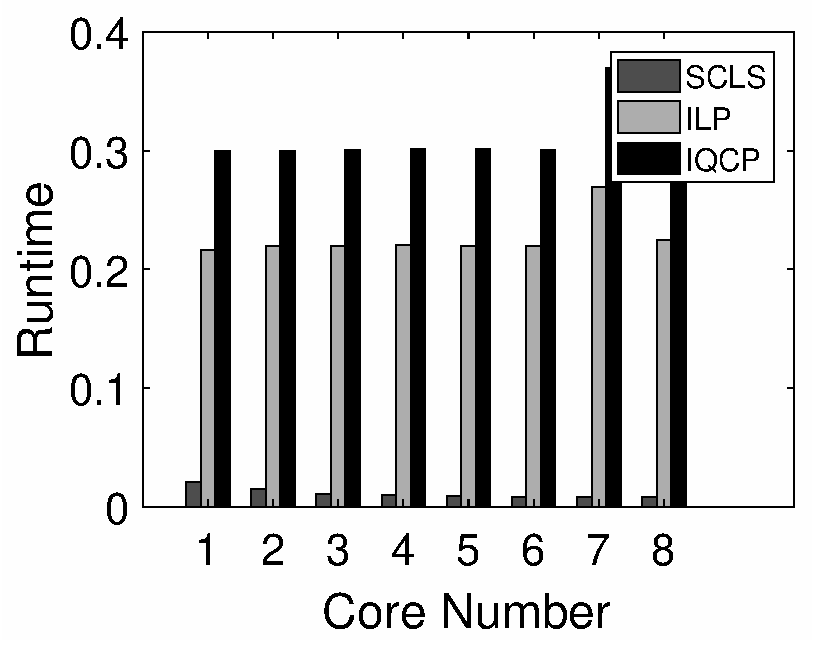
\includegraphics[width=0.22\textwidth]{franz/Runtime_noKSP_noCOSE}}
%\end{figure*}
%
%
%\begin{figure*}[tp]
%\centering
\subfigure[Efficiency]{
\label{fig:Efficiency}
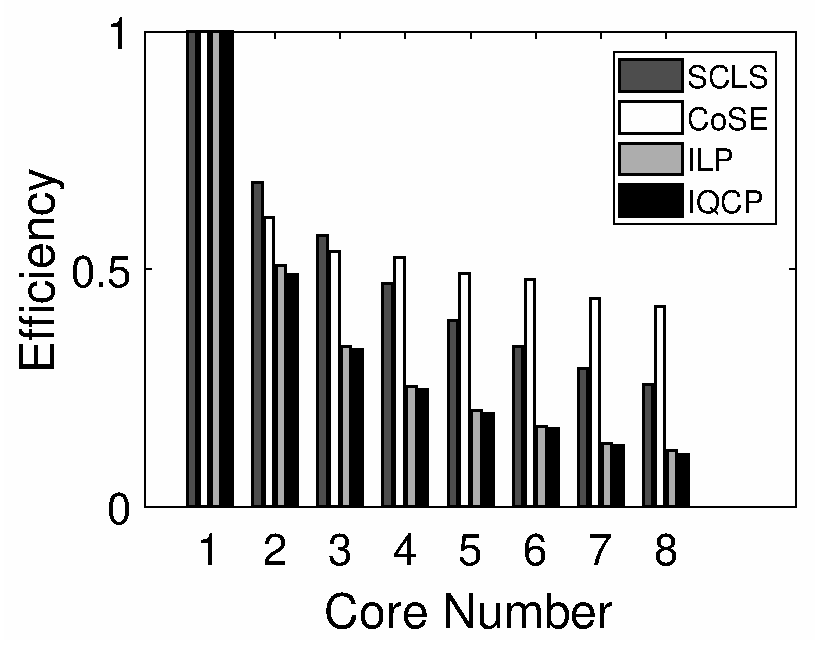
\includegraphics[width=0.22\textwidth]{franz/Efficiency}}
\subfigure[Core speedup]{
\label{fig:Speedup}
\includegraphics[width=0.22\textwidth]{franz/speedup}}
\subfigure[Algorithm speedup]{
\label{fig:Multiple}
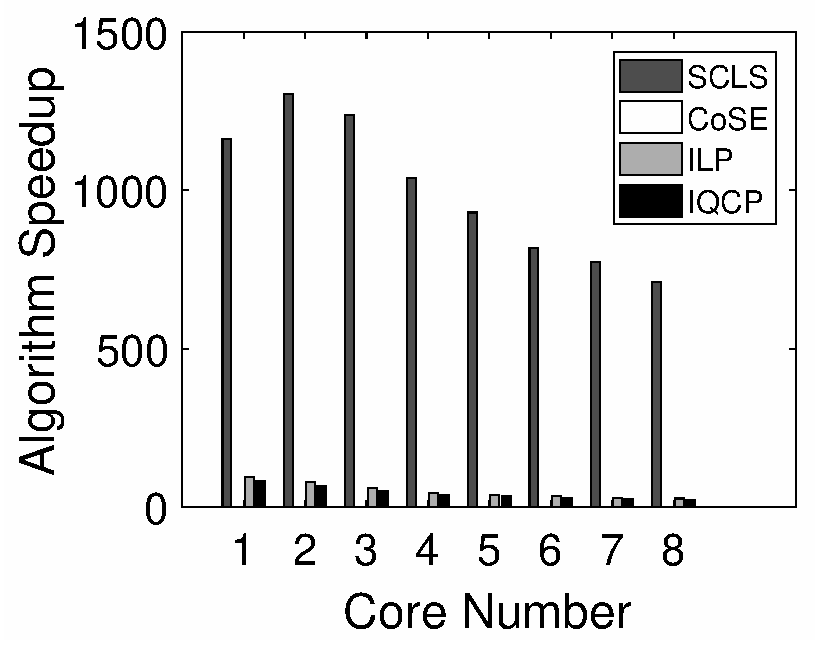
\includegraphics[width=0.22\textwidth]{franz/Multiple}}
\subfigure[Algorithm speedup without SCLS]{
\label{fig:MultipleNoSCLS}
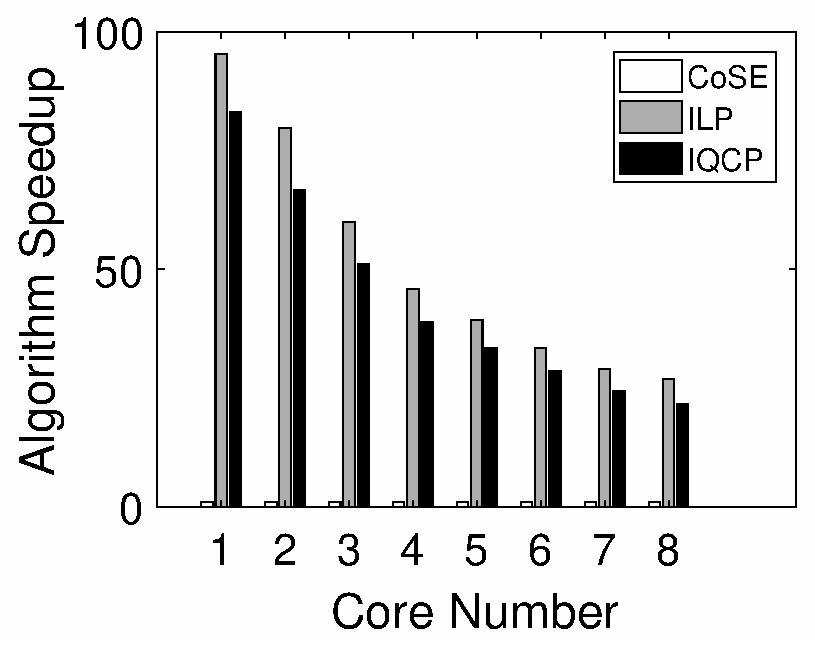
\includegraphics[width=0.22\textwidth]{franz/MultipleNoSCLS}}
\caption{Simulation results of finding the SRLG disjoint paths}
\label{fig:SLNGExperimentalData}
\end{figure*}

\begin{itemize}
  \item Path Hop
\end{itemize}


Fig.\ref{fig:normalization hop} shows the path hop of AP, BP, and the sum of both AP and BP. As all algorithms target to minimize the least path weight of the SRLG-disjoint path pair instead of the number of path hops, they have the same AP weight (Fig.\ref{fig:normalization weitgh sum}) even though they have different AP path hops (Fig.\ref{fig:normalization hop}). Although the AP weights under all algorithms are smaller than the BP weights in Fig.\ref{fig:normalization weitgh sum}, in Fig.\ref{fig:normalization hop}, the AP hops may not always be fewer than the BP hops.

\begin{itemize}
  \item Runtime
\end{itemize}


\label{subsubsec:Runtime}
Fig.\ref{fig:normalization runtime} shows the run time under different algorithms by varying the number of CPU cores utilized.
As the runtime under CoSE is significantly larger than that under other algorithms, to more clearly show the results of other algorithms, we further plot the runtime results in Fig.\ref{fig:Runtime_noKSP_noCOSE} by excluding CoSE.
As ILP, and IQCP are not parallel algorithms, the runtime of these algorithms under different number of cores is approximately equal. The runtime of our SCLS  and CoSE decreases with the increase of the number of processor cores because these two algorithms can partition the original problem into multiple sub-problems to execute in parallel and take advantage of the parallelism of the multi-core CPU to speed up the path searching process. Although CoSE is a parallel algorithm, the computation time is even larger than  ILP and IQCP. Some possible reasons include 1) the search process to find the conflicting SRLG set in CoSE  is not efficient; 2) As one SRLG usually includes multiple links, the partitioning of problem based on conflicting SRLG will introduce a large number of sub-problems to solve, which also results in a large computation cost.

Different from CoSE, our SCLS looks for the set of conflicting links on an AP caught into the trap problem based on the min-cut theory in graph, and achieves the lowest time in Fig.\ref{fig:normalization runtime}. This demonstrates that our conflicting link set finding algorithm is efficient, and moreover our divide-and-conquer algorithm and intelligent AP searching process based on SRLG Conflicting Link Set can largely reduce the computation cost.

%KSP is known as an effective algorithm to handle the trap problem. However, among all the algorithms implemented, the running time under KSP is the largest. A major problem of KSP is that after the current candidate AP fails the test (that is, it does not have a corresponding disjoint BP), the next candidate AP to be tested is selected solely based on the path length. In the 8 topologies we studied in the trace,  usually a large number of paths need to be tested in order to find a disjoint path pair (if it exists between a pair of nodes), thus KSP needs a large computation time.

\begin{itemize}
  \item Algorithm speedup
\end{itemize}


In Fig.\ref{fig:Multiple}, we further compare their computation speeds. Specially, to find out how much speedup is gained when using different algorithms to find the required paths,to calculate the algorithm speedup metric,we use CoSE as the baseline algorithm and set $alg_1$ =CoSE. Similar to the results in the Fig.\ref{fig:normalization runtime}, the speed of SCLS is more than 1000 times that of  CoSE in Fig.\ref{fig:Multiple}.  Similar to Fig.\ref{fig:normalization runtime}, as the running speed of CoSE is significantly smaller than others and can hardly be observed in Fig.\ref{fig:Multiple}, we further plot the algorithm speedup results in Fig.\ref{fig:MultipleNoSCLS} by excluding the largest one SCLS.

\begin{itemize}
  \item Core speedup
\end{itemize}

Rather than using the algorithm speedup to compare the overall running speeds of all algorithms, the metric "core speedup" is utilized to evaluate how the number of cores in the CPU impacts the running speed of a given algorithm.
Fig.\ref{fig:Speedup} plots the core speedup under all algorithms implemented.
%For the two parallel algorithms SCLS and CoSE, the core speedup   increases with the increase of the number of cores. %\del{Therefore, larger number of cores brings larger performance gain for these two parallel algorithms SCLS and CoSE.}
%However, the increasing speed becomes smaller when the number of cores becomes larger and it incurs a higher cost to coordinate the process.
Core speedup under algorithms ILP and IQCP is  approximately equal to 1 under any core number because they are not parallel algorithms. The core speedup of our SCLS increases with increase of core number when it is less than 4, beyond which the core speedup of SCLS remains stable, which demonstrates that 4 core is sufficient for SCLS. This result is consistent with Amdahl's law \cite{amdahl1967validity} that the theoretical core speedup is limited to a upper bound determined by the problem size. However, the core speed under CoSE continues to increases even though the core number is  equal to 8 which doubles the number 4. This result demonstrates that even 8-core CPU can not satisfy the parallelism requirement in CoSE. This is because the conflicting SRLG set found by CoSE includes  a large number of links,  which further results in a large number of sub-problems  and thus large problem size and  computation cost.


%1) the search
%process to find the conflicting SRLG set in CoSE is not
%efficient; 2) As one SRLG usually includes multiple links,
%the partitioning of problem based on conflicting SRLG will
%introduce a large number of sub-problems to solve, which also
%results in a large computation cost
%
%Among all algorithms, \revtao{the core speedup of our SCLS is the largest except CoSE, which demonstrates that our divide and conquer algorithm designed  based on the SRLG conflicting link set can bring the largest parallelism gain than non-parallel algorithm, and the cardinality of subproblem is smaller than CoSE}.

%\note{How many paths pairs to search in your simulations. If you only search for one pair, then the sub=-problems may be lower than the number of cores, so multi core cannot be used.}
\begin{itemize}
  \item Efficiency
\end{itemize}


Efficiency is a measure of the overhead due to the parallelization. Programs with a high efficiency spend more time on useful work and less time on synchronization and communications.Similar to Fig.\ref{fig:Speedup}, with more cores involved, the efficiency value decreases  as a large core number brings more cost to coordinate the process. In Fig.\ref{fig:Efficiency}, the efficiency values of all algorithms decrease with the increase of the core number. Consistent with the results in Fig.\ref{fig:Speedup}, as CoSE introduces more sub-problems than our SCLS, after the core number reaches 4, the efficiency under CoSE is larger than SCLS. However, our SCLS achieves significantly larger algorithm speedup as shown Fig.\ref{fig:Multiple}. %\note{You'd better use the same colore to represent the same algorithm in different figures. It makes reading and understanding difficult with your messy color setup. You may explain what is algorithm speedup and core speedup earlier when you first refer them, although you don't need to give formal definition.}

All the simulation results demonstrate that our SCLS can outperform other approaches with higher routing performance while at a much higher search speed, because the  conflicting link set found can facilitate efficient problem partition for parallel algorithm execution with low computation cost.

\subsection{Simulation of finding the SRNG disjoint paths}
In this section, we present our simulation result \rev{for the extension of our} SCLS to find the node-disjoint routing paths. Similar to the simulation setup in Section \ref{subsub:Simulation setup}, we inject SRNGs into a topology trace published. Each SRNG group is generated by randomly selecting 2-5 nodes. Table \ref{tab:AllSample1} shows the basic network setting (number of nodes, links) in these 7 topologies after injecting SRNGs.

As discussed in Section \ref{sec:Extension to the risk sharing among nodes}, through  node splitting,  a node-disjoint routing problem could be transformed into a link-disjoint routing problem. Besides our SCLS, we also implement other four SRLG-disjoint routing algorithms (ILP, IQCP, KSP, CoSE) for performance comparison.

Fig.\ref{fig:SRNGExperimentalData} shows the simulation results of finding the SRNG disjoint paths. Fig.\ref{fig:SRNGExperimentalData} \rev{shows similar results as those in}  Section \ref{subsubsec:Simulation result}. All the simulation results demonstrate that our SCLS is feasible for all the network scenarios (both SRLG and SRNG), and can outperform other approaches with higher routing performance while at a much higher search speed.


\begin{table*}[htbp]
\caption{$\TopoNum$ different topologies.}
  \centering
\footnotesize{  \begin{tabular}{*{18}{c}}
\toprule
Topology & 1 & 2 & 3 & 4 & 5 & 6& 7   \\
\midrule
Node    &     865&      738    &      740     &    2566             &     988     &     831     &     687       \\
Edge   &    4496 &  4269     &    4371      &   4685          &       3317   &      4362   &      3016    \\
%Graph density  & 1.5\% &    1.49\% &   1.52\%  &  0.1\%  &   0.10\% &   1.41\%  &  1.5\% &   1.38\%   \\
No.SRNG & 113 &  75   &  77  &  184        & 184  &  102  &   83    \\
SRNG node ratio & 39.08\% & 29.40\% &   29.86\% &   21.16\%    &   54.35\%  &  37.30\% &   35.23\%     \\
\bottomrule
\end{tabular}
}

\label{tab:AllSample1}
\end{table*}



\begin{figure*}[htbp]
\centering
\subfigure[Path weight]{
\label{fig:Nodenormalization weitgh sum}
\includegraphics[width=0.22\textwidth]{franz/Nodeweight}}
\subfigure[Path hop]{
\label{fig:Nodenormalization hop}
\includegraphics[width=0.22\textwidth]{franz/Nodehop}}
\subfigure[Runtime]{
\label{fig:Nodenormalization runtime}
\includegraphics[width=0.22\textwidth]{franz/Noderuntime}}
\subfigure[Runtime without CoSE]{
\label{fig:NodeRuntime_noKSP_noCOSE}
\includegraphics[width=0.22\textwidth]{franz/NodeRuntime_noKSP_noCOSE}}
%\end{figure*}
%
%
%\begin{figure*}[tp]
%\centering
\subfigure[Efficiency]{
\label{fig:NodeEfficiency}
\includegraphics[width=0.22\textwidth]{franz/NodeEfficiency}}
\subfigure[Core speedup]{
\label{fig:NodeSpeedup}
\includegraphics[width=0.22\textwidth]{franz/Nodespeedup}}
\subfigure[Algorithm speedup]{
\label{fig:NodeMultiple}
\includegraphics[width=0.22\textwidth]{franz/NodeMultiple}}
\subfigure[Algorithm speedup without SCLS]{
\label{fig:NodeMultipleNoSCLS}
\includegraphics[width=0.22\textwidth]{franz/NodeMultipleNoSCLS}}
\caption{Simulation results of finding the SRNG disjoint paths}
\label{fig:SRNGExperimentalData}
\end{figure*}


%\rev{ The low-efficiency of CoSE dividing and conquer initial problem make the scale of sub-problems is relative enormous, so that problem size of CoSE is much larger than SCLS, therefore performance of the speedup and efficiency of CoSE is more than SCLS when core number exceed than four \cite{grama2003introduction}}
% Among all algorithms, \revtao{the efficiency value of our SCLS is the largest under different core numbers, which demonstrates that our divide and conquer algorithm designed  based on the SRLG conflicting link set can bring the largest parallelism gain than other all non-parallel algorithms.}
%
%
%
% \begin{figure}
%   \centering
%   % Requires \usepackage{graphicx}
%   \includegraphics[width=2.35in]{franz/runtime_nocose}\\
%   \caption{Normalization Runtime without CoSE value}\label{fig:normalization runtime_nocose}
% \end{figure}
%
%
% \subsubsection{Speed}
% The speedupSCLSte{bryant2003computer} of a parallel program is typically defined as
%  \begin{equation}\label{equ:speed}
%    S_P=\frac{T_1}{T_p}
% \end{equation}
% where p is the number of processor cores and $T_k$ is the running time on k cores.Calculating the speedup of every processor cores in all algorithms in Fig.\ref{fig:Speedup} by the runtime of all algorithm from Fig.\ref{fig:normalization runtime}. The speedup value of CoSE increase with increasing the number of processor cores. The speedup value of CSLIE firstly increase then decrease because four cores is neck bottle of parallelism for CSLIE heuristic in this samples. The speedup value of other algorithm is affected slightly by the number of core processors.
%\begin{figure}
%  \centering
%  % Requires \usepackage{graphicx}
%  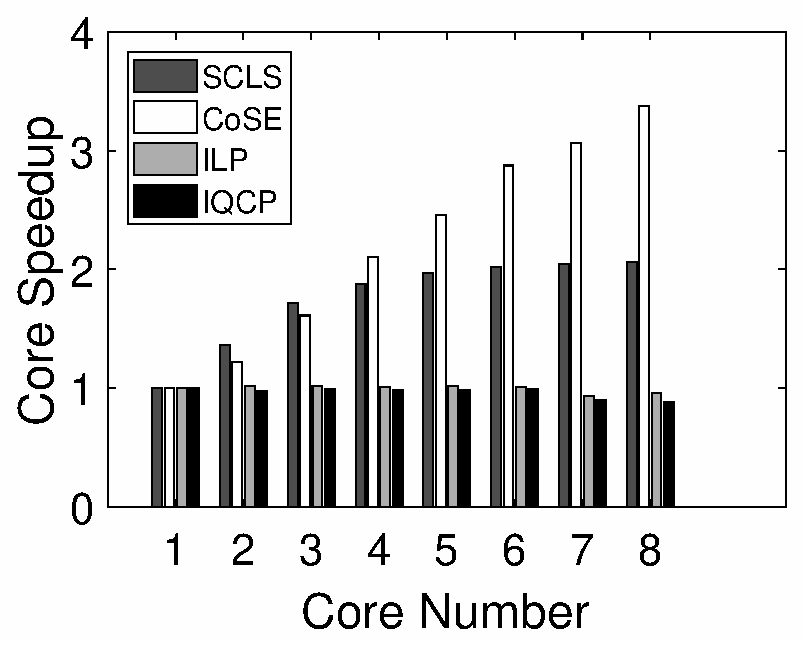
\includegraphics[width=2.35in]{franz/Speedup}\\
%  \caption{Speedup}\label{fig:Speedup}
%\end{figure}
%
%
%\subsubsection{Efficient}
%A related measureSCLSte{bryant2003computer} in Fig.\ref{fig:Efficiency}, known as efficiency, is defined as
%\begin{equation}\label{equ:efficient}
%  E_p=\frac{S_p}{p}=\frac{T_1}{pT_p}
%\end{equation}
%and is typically reported as a percentage in the range (0, 100]. Efficiency is a measure of the overhead due to parallelization. Programs with high efficiency are spending more time doing useful work and less time synchronizing and communicating than programs with low efficiency. Efficiet value of all algorithm decrease with the increase of core processors.
%\begin{figure}
%  \centering
%  % Requires \usepackage{graphicx}
%  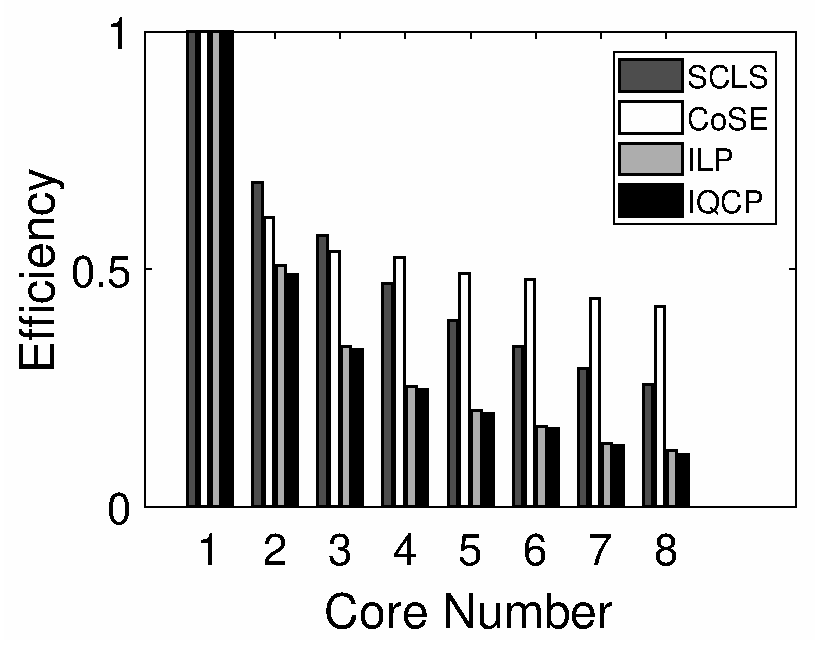
\includegraphics[width=2.35in]{franz/Efficiency}\\
%  \caption{Efficiency}\label{fig:Efficiency}
%\end{figure}
%\subsubsection{Multiple}
%The multiple's definition of parallel typically defined as
%\begin{equation}\label{equ:multiple}
%  M_n^x=\frac{T_n^{ILP}}{T_n^x}
%\end{equation}
%where x is algorithm such as CSLIE,CoSE,KSP ILP and IQCP. $T_n^x$ is the runtime of x algorithm in n processor cores. $T_n^{ILP}$ is the runtime of ILP in n processor cores. All algorithm compares with ILP runtime in Fig.\ref{fig:Multiple}

